\documentclass[11pt,a4paper]{article}

\usepackage[a4paper,left=2.2cm,right=2.2cm,top=2.1cm,bottom=2.3cm]{geometry}
\usepackage{fontspec}
\usepackage[table]{xcolor}
\usepackage{graphicx}
\usepackage{booktabs}
\usepackage{array}
\usepackage{tabularx}
\usepackage{titlesec}
\usepackage{caption}
\usepackage{enumitem}
\usepackage{float}
\usepackage{fancyhdr}
\usepackage{microtype}
\usepackage[hidelinks]{hyperref}

\setmainfont{Charter}[BoldFont={Charter Bold},ItalicFont={Charter Italic},BoldItalicFont={Charter Bold Italic}]
\newfontfamily\headfont{Avenir Next}[Ligatures=TeX,UprightFont={* Medium},BoldFont={* Demi Bold},ItalicFont={* Medium Italic}]
\newfontfamily\headfontreg{Avenir Next}[Ligatures=TeX,UprightFont={* Regular}]
\setmonofont{Menlo}[Scale=0.8]
\newfontfamily\devfont[Script=Devanagari]{Devanagari Sangam MN}
\newcommand{\hi}[1]{{\devfont #1}}
\newcommand{\nAblDenseVerify}{0.829}
\newcommand{\nAblFull}{0.843}
\newcommand{\nAblNoAlign}{0.408}
\newcommand{\nAblNoDates}{0.851}
\newcommand{\nAblNoDf}{0.727}
\newcommand{\nAblNoNames}{0.759}
\newcommand{\nAblNoNumbers}{0.844}
\newcommand{\nAblTranslitExact}{0.791}
\newcommand{\nBnF}{0.133}
\newcommand{\nBnPone}{0.917}
\newcommand{\nBtBmSeo}{0.637}
\newcommand{\nBtBmSum}{0.642}
\newcommand{\nBtBmTrans}{0.700}
\newcommand{\nBtLlmSec}{17.4}
\newcommand{\nBtSpinFprAbsent}{0.000}
\newcommand{\nBtSpinFprSame}{0.060}
\newcommand{\nBtSpinFprShort}{0.120}
\newcommand{\nBtSpinPone}{0.993}
\newcommand{\nBtSpinSeo}{0.771}
\newcommand{\nBtSpinSum}{0.753}
\newcommand{\nBtSpinTrans}{0.906}
\newcommand{\nBtTfidfPone}{1.000}
\newcommand{\nBtTfidfSeo}{0.800}
\newcommand{\nBtTfidfSum}{0.427}
\newcommand{\nBtTfidfTrans}{0.897}
\newcommand{\nCrawlAllReq}{62{,}861}
\newcommand{\nCrawlAudited}{62{,}852}
\newcommand{\nCrawlBack}{33}
\newcommand{\nCrawlDisallowed}{0}
\newcommand{\nCrawlDocs}{13{,}299}
\newcommand{\nCrawlGap}{20.0}
\newcommand{\nCrawlHosts}{45}
\newcommand{\nCrawlReq}{17{,}688}
\newcommand{\nCrawlRobots}{146}
\newcommand{\nCrawlSkips}{4{,}695}
\newcommand{\nCrawlTrap}{298}
\newcommand{\nCrawlUnder}{0}
\newcommand{\nDenseBnPone}{0.083}
\newcommand{\nDenseFprAbsent}{0.209}
\newcommand{\nDenseFprSame}{0.720}
\newcommand{\nDenseFprShort}{0.700}
\newcommand{\nDenseMs}{26}
\newcommand{\nDensePone}{0.926}
\newcommand{\nDenseSeo}{0.383}
\newcommand{\nDenseSum}{0.385}
\newcommand{\nDenseTaPone}{0.083}
\newcommand{\nDenseTePone}{0.083}
\newcommand{\nDenseTrans}{0.410}
\newcommand{\nDocsCrawl}{46{,}479}
\newcommand{\nIndic}{2{,}329}
\newcommand{\nLatinSum}{0.163}
\newcommand{\nLenAucSeo}{0.73}
\newcommand{\nLenAucSum}{1.00}
\newcommand{\nLenAucSumShort}{0.72}
\newcommand{\nLenAucTrans}{0.54}
\newcommand{\nLenLongMed}{229}
\newcommand{\nLenShortMed}{130}
\newcommand{\nLenSumMed}{116}
\newcommand{\nMsAblFull}{0.870}
\newcommand{\nMsAblNoResid}{0.844}
\newcommand{\nMsAll}{0.870}
\newcommand{\nMsContAll}{0.742}
\newcommand{\nMsFalseSame}{0.078}
\newcommand{\nMsFalseSameMid}{0.156}
\newcommand{\nMsLlm}{0.507}
\newcommand{\nMsLlmCont}{0.035}
\newcommand{\nMsLlmPrec}{1.000}
\newcommand{\nMsLlmRecall}{0.339}
\newcommand{\nMsMidAll}{0.117}
\newcommand{\nMsMinhashAll}{0.188}
\newcommand{\nMsMs}{99}
\newcommand{\nMsPlain}{1.000}
\newcommand{\nMsPlainCont}{0.981}
\newcommand{\nMsSecondMid}{0.036}
\newcommand{\nMsSecondSpin}{0.812}
\newcommand{\nMsSeo}{0.329}
\newcommand{\nMsSeoCont}{0.050}
\newcommand{\nMsSyn}{0.938}
\newcommand{\nMsSynCont}{0.582}
\newcommand{\nMsThirdMid}{0.000}
\newcommand{\nMsThirdSpin}{0.705}
\newcommand{\nSameSiteFlagged}{2}
\newcommand{\nSameSiteSuspects}{299}
\newcommand{\nSites}{37}
\newcommand{\nSpeedup}{36}
\newcommand{\nTaF}{0.000}
\newcommand{\nTaPone}{0.417}
\newcommand{\nTeF}{0.000}
\newcommand{\nTePone}{0.667}
\newcommand{\nXlColdMs}{483}
\newcommand{\nXlFprAbsent}{0.000}
\newcommand{\nXlFprSame}{0.100}
\newcommand{\nXlFprShort}{0.220}
\newcommand{\nXlLiveAgency}{1}
\newcommand{\nXlLiveCredit}{2}
\newcommand{\nXlLiveDeva}{2{,}136}
\newcommand{\nXlLiveFlagged}{15}
\newcommand{\nXlLiveLag}{3.5}
\newcommand{\nXlLiveSuspects}{2{,}375}
\newcommand{\nXlMs}{65}
\newcommand{\nXlPone}{0.993}
\newcommand{\nXlPostings}{68483}
\newcommand{\nXlRetMs}{15}
\newcommand{\nXlSeo}{0.852}
\newcommand{\nXlSum}{0.818}
\newcommand{\nXlTestN}{49}
\newcommand{\nXlTrans}{0.860}
\newcommand{\nXlmBlock}{3}
\newcommand{\nXlmExact}{0.387}
\newcommand{\nXlmF}{0.765}
\newcommand{\nXlmFalseSame}{0.300}
\newcommand{\nXlmFalseShort}{0.280}
\newcommand{\nXlmMs}{103}
\newcommand{\nXlmN}{142}
\newcommand{\nXlmPrec}{1.000}
\newcommand{\nXlmRecall}{0.620}
\newcommand{\nXlmSummaryFound}{0.673}
\newcommand{\nXlmWholeF}{0.528}
\newcommand{\nXlmWholeFalseSame}{0.100}
\newcommand{\nXlmWholeFalseShort}{0.240}
\newcommand{\nXlmWholePrec}{1.000}
\newcommand{\nXlmWholeRecall}{0.359}
\newcommand{\nXlmWholeSummaryFound}{0.918}


\definecolor{ink}{HTML}{1E1C1A}
\definecolor{oxblood}{HTML}{7A2E2E}
\definecolor{ochre}{HTML}{B5832A}
\definecolor{olive}{HTML}{5F6B3A}
\definecolor{warmgrey}{HTML}{8A837A}
\definecolor{paper}{HTML}{F3EFE7}
\definecolor{ourrow}{HTML}{F5ECE9}
\color{ink}

\hypersetup{colorlinks=true,linkcolor=oxblood,citecolor=oxblood,urlcolor=oxblood,
  pdftitle={SpinTrace: tracing rewritten, translated and stitched news to its sources},pdfauthor={CSD358 team}}

\linespread{1.03}
\setlength{\parindent}{0pt}
\setlength{\parskip}{0.4em}
\frenchspacing

\titleformat{\section}{\headfont\bfseries\large\color{ink}}{\thesection}{0.7em}{}[\vspace{0.1em}{\color{oxblood}\titlerule[0.5pt]}]
\titlespacing*{\section}{0pt}{1.1em}{0.5em}
\titleformat{\subsection}{\headfont\bfseries\normalsize\color{ink}}{\thesubsection}{0.6em}{}
\titlespacing*{\subsection}{0pt}{0.9em}{0.15em}
\titleformat{\paragraph}[runin]{\headfont\bfseries\small\color{ink}}{}{0pt}{}[.]
\titlespacing*{\paragraph}{0pt}{0.5em}{0.6em}

\captionsetup{font={small},labelfont={color=oxblood},textfont={},labelsep=period,skip=5pt,
  justification=raggedright,singlelinecheck=false}
\DeclareCaptionFont{avenir}{\headfontreg}
\captionsetup{font={avenir,small}}
\setlength{\textfloatsep}{12pt plus 2pt minus 2pt}
\setlength{\floatsep}{10pt plus 2pt minus 2pt}

\setlist{itemsep=0.15em,topsep=0.2em,parsep=0pt,leftmargin=1.4em}

\pagestyle{fancy}
\fancyhf{}
\renewcommand{\headrulewidth}{0pt}
\fancyfoot[C]{\headfontreg\footnotesize\color{warmgrey}\thepage}

% tables: Avenir header on a paper tint, hairline rules, our method's row tinted
\setlength{\aboverulesep}{0.25ex}
\setlength{\belowrulesep}{0.35ex}
\setlength{\heavyrulewidth}{0.6pt}
\setlength{\lightrulewidth}{0.35pt}
\arrayrulecolor{warmgrey}
\newcommand{\hd}[1]{{\headfont\bfseries\footnotesize #1}}
\newcommand{\hrow}{\rowcolor{paper}}
\newcommand{\ours}{\rowcolor{ourrow}}
\newcommand{\code}[1]{\texttt{#1}}
\newcolumntype{R}{>{\raggedleft\arraybackslash}X}
\newcolumntype{P}[1]{>{\raggedright\arraybackslash}p{#1}}
\newcolumntype{L}{>{\raggedright\arraybackslash}X}
\newenvironment{wdlist}{\begin{minipage}[t]{\linewidth}\raggedright\vspace{1pt}\begin{itemize}[leftmargin=1.1em,label=\textbullet,itemsep=3.5pt,topsep=0pt,parsep=0pt,partopsep=0pt]}{\end{itemize}\vspace{5pt}\end{minipage}}
\newcommand{\hdd}[2]{\hd{\begin{tabular}[b]{@{}r@{}}#1\\#2\end{tabular}}}

\begin{document}

{\headfont\bfseries\LARGE SpinTrace\par}
\vspace{0.25em}
{\headfont\large Tracing rewritten, translated and stitched news to its sources\par}
\vspace{0.7em}
{\headfontreg\small Nishita Kadali\quad\textcolor{warmgrey}{/}\quad Pustak Pathak\par
CSD358 Information Retrieval, final project, Track 4: web crawling, freshness and web integrity\par
November 2026\par}
\vspace{0.4em}

\section{Problem and track relevance}

In August 2023 NewsGuard gave 43 AI-rewritten articles from content farms to Grammarly's premium plagiarism checker. It could not identify the original source of 34 of them, a 79\% failure rate~\cite{ng2023}. The farms take a story from a mainstream outlet, have a language model reword it, and publish the result as their own. NewsGuard's tracking page now counts 3,749 AI content-farm sites~\cite{ng2026}. The checker fails for a structural reason: it looks for text pulled verbatim, and a paraphrase has very little of it.

A web crawler has the same blind spot. Its ``content seen?'' check fingerprints each page and compares sets of word shingles, which catches mirrors and light edits~\cite{broder1997,manku2007,iir2008}. A paraphrase shares almost no word 5-grams with its source; in our tests MinHash Jaccard reaches an F1 of 0.021 on SEO-style rewrites (Section~\ref{sec:eval}). The crawler then indexes the rewrite as new content, and in search the copy competes with the article it was taken from.

We had two users in mind. One runs a crawler or a search index and wants to know, when a page arrives, whether it is derived from a page already stored, which page that is, and how to keep the original above its copies in the ranking. The other is an editor or fact-checker holding one suspicious article who wants its likely source and the evidence: the sentences that align and the names, numbers and quotes the two share.

Track~4 asks for a focused crawler and a small index that address one integrity problem end to end, and it names the content-seen check, near-duplicate detection and politeness as hooks. Its first sample idea is a news crawler that detects near-duplicate and rewritten articles. We started there and changed what counts as ``seen'': SpinTrace extends the crawler's content-seen check from copy detection to paraphrase-aware derivative detection. It retrieves a rewrite's likely source using the facts a rewrite rarely changes, then traces provenance and demotes copies in ranking. The work we built on is Broder's resemblance and containment~\cite{broder1997}, Manku et al.\ on near-duplicates in a production crawler~\cite{manku2007}, the Mercator frontier~\cite{heydon1999}, the textbook treatment of scoring and index elimination~\cite{iir2008}, BM25~\cite{robertson2009} and Sentence-BERT~\cite{reimers2019}.

\paragraph{What the final project adds} The mid-term system, like every copy detector we know of, assumes that a derivative shares wording with one original. Two kinds of derivative break that assumption, and a content farm has reason to produce both. A \emph{translation} shares no words with its source at all. A \emph{mashup} stitches one article from two or three originals, so no single original explains it, and a detector that returns its best match finds one source and stops. The final project traces both to their originals. The premise is unchanged: a rewrite or a translation changes the wording but keeps the names, numbers and dates, which stay high-idf evidence in the crawler's own index. We extend what counts as evidence across scripts (numbers, dates and names written in Devanagari, Bengali, Tamil and other Indian scripts) and what counts as a query (the sentences of the suspect that no source has explained yet).

\section{How we used IR}

Our premise is that a rewrite changes the wording but keeps the names, numbers, dates and direct quotes. In IR terms those are high-idf terms and exact phrases. So the classical machinery (an inverted index, idf weights, positional phrase queries and a date filter) finds the candidate sources, and a sentence-embedding model only checks the few candidates IR returns. Figure~\ref{fig:pipeline} shows the pipeline. Table~\ref{tab:concepts} groups the concepts we use under the assignment's five lecture topics and points to the code; the paragraphs below give the choices and the reasons.

\begin{figure}[t]
  \centering
  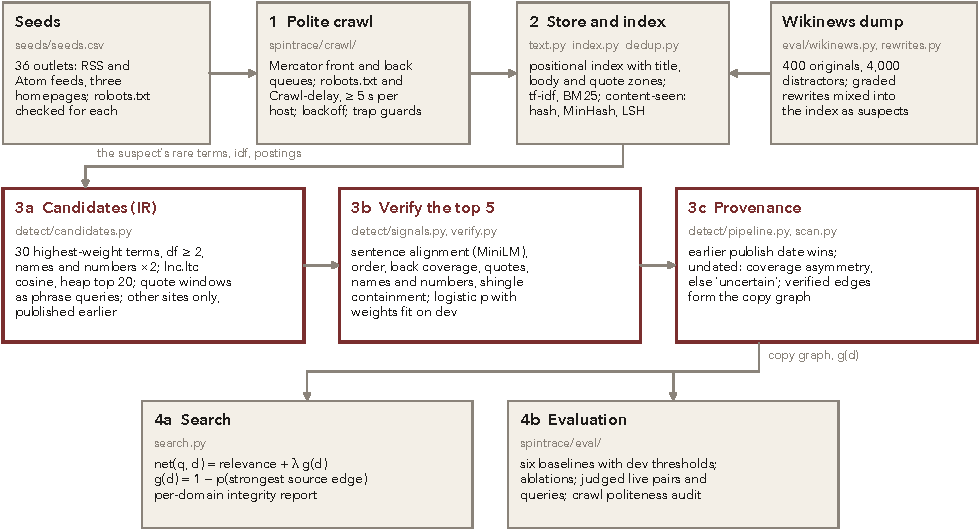
\includegraphics[width=0.94\textwidth]{figures/pipeline.pdf}
  \caption{The SpinTrace pipeline. Oxblood boxes are the detection stage that extends the content-seen check; paths are under \code{spintrace/}.}
  \label{fig:pipeline}
\end{figure}

\begin{table}[t]
  \centering\small
  \caption{IR concepts in SpinTrace, grouped by the five lecture topics listed in the assignment. Code paths are under \code{spintrace/}. Outside the syllabus, BM25 and dense retrieval serve as baselines (\code{index.py}, \code{eval/run.py}).}
  \label{tab:concepts}
  \footnotesize
  \begin{tabularx}{\textwidth}{@{}P{2.5cm}P{5.4cm}LP{3.2cm}@{}}
    \toprule
    \hrow \hd{Lecture topic} & \hd{Concepts we use} & \hd{Why SpinTrace needs them} & \hd{Code} \\
    \midrule
    {\headfont Boolean retrieval} & Inverted index (dictionary and postings); postings intersection in increasing df order & Phrase queries and the candidate query both walk postings lists & \code{index.py} \\
    \addlinespace[2pt]
    {\headfont Term vocabulary and postings} & Tokenisation, case and accent folding, numbers as values; Porter stemming, compared with none; positional index and phrase queries; precision and recall & One pipeline for index, shingles and queries; quotes survive rewriting, so they become phrase queries & \code{text.py}\newline\code{index.py}\newline\code{eval/report.py} \\
    \addlinespace[2pt]
    {\headfont tf-idf and the vector space model} & Jaccard over shingles; idf; lnc.ltc tf-idf; cosine with length normalisation & Jaccard is the check we extend; rare terms carry the evidence; summaries are short, so length normalisation matters & \code{dedup.py}\newline\code{index.py} \\
    \addlinespace[2pt]
    {\headfont Scoring and result assembly} & Index elimination (high-idf terms) with heap top-K; title, body and quote zones; parametric filter on publish date; static quality g(d) and net score & Query only the terms a rewrite keeps; a source must be published first; originals should rank above their copies & \code{detect/candidates.py}\newline\code{detect/scan.py}\newline\code{search.py} \\
    \addlinespace[2pt]
    {\headfont Web crawling} & Crawl loop, Mercator front and back queues, politeness, robots.txt; URL normalisation and spider-trap guards; content-seen check (hash, MinHash, LSH); freshness by re-polling feeds & Collect news without burdening sites; the content-seen check is what SpinTrace extends & \code{crawl/}\newline\code{dedup.py} \\
    \addlinespace[2pt]
    {\headfont Tolerant retrieval and feedback} & Character k-gram index over phonetic name keys, with Jaccard overlap and edit distance; a query reformulated from the part of the suspect no source explains yet & Names change spelling across scripts; a second source hides behind the first until its own sentences are queried & \code{kgram.py}, \code{detect/crosslingual.py}, \code{detect/multisource.py} \\
    \bottomrule
  \end{tabularx}
\end{table}

\paragraph{Crawl} \code{crawl/frontier.py} follows Mercator's split between front queues for priority and back queues for politeness~\cite{heydon1999}. Each host keeps three priority levels (feed and sitemap entries, article-shaped links, everything else) drawn with bias 8:3:1, and a heap of next-allowed fetch times picks the host. Priority sits in one function, \code{priority()}, so a farm-aware policy can replace it later. \code{crawl/robots.py} fetches and stores robots.txt per host and obeys Crawl-delay. The delay is max(Crawl-delay,~5\,s), enforced by the heap and again by a guard before every request. A 5xx, a 429 or a refusal (401, 403, 405, 451) doubles the delay, Retry-After is honoured, and a host is dropped after 5 consecutive errors. Redirects are not followed automatically, so a redirect target goes back through robots.txt and the delay. \code{crawl/urlnorm.py} lowercases the host, drops fragments and tracking parameters and sorts the query. Trap guards reject long, deep, repetitive or parameter-heavy URLs and cap a host at 1,500 pages. A document is trafilatura's main text of at least 120 words plus a publish date from page metadata or the feed. The date matters later, for provenance.

\paragraph{Text and index} \code{text.py} is the one normalisation pipeline for the index, the shingles and the queries: NFKC, case and accent folding, and numbers kept as values so that ``1,394'' matches ``1394''. Stopwords stay in the postings because phrase queries need every position. \code{index.py} builds a positional index with three zones (title, body, quote) and computes lnc.ltc tf-idf and BM25 (\textit{k}\textsubscript{1}~=~1.2, \textit{b}~=~0.75). Phrase queries intersect postings in increasing df order.

\paragraph{Content-seen check} \code{dedup.py} is the textbook check that SpinTrace extends: an exact hash of the normalised text, word 5-gram shingles, MinHash with 128 permutations (estimate error about 0.09) and LSH with 32 bands of 4 rows, whose knee at Jaccard 0.42 catches light edits~\cite{broder1997,iir2008}. It stays in the crawler and runs first. It is also the baseline we have to beat.

\paragraph{Rare-term candidate query} \code{detect/candidates.py} turns a suspect into a query of its 30 highest-weight body terms with df~≥~2, boosting names and numbers by 2. This is index elimination in the textbook sense~\cite[ch.~7]{iir2008}: only the postings of high-idf terms are walked, scores accumulate term at a time, and a heap returns the top 20. Terms with df~=~1 are left out because they can only match the suspect itself. We score with lnc.ltc because it puts idf on the query side only, so the rare terms decide, and cosine length normalisation keeps long articles from winning, which matters when the suspect is a short summary. Quotes are cut into 6-token windows (step 3) and run as phrase queries on the positional index; a rewrite may trim a quote, and any intact window is evidence. A parametric filter keeps only documents from other sites published before the suspect.

\paragraph{Verification} \code{detect/signals.py} and \code{detect/verify.py} check the top 5 candidates. Each signal is an independent scorer: sentence alignment coverage (two sentences match at MiniLM cosine ≥~0.62), the mean alignment score, whether aligned sentences keep their order, back coverage of the candidate, word overlap inside aligned pairs, quote overlap, overlap of names and numbers, shingle containment and the rare-term cosine from retrieval. A class-balanced logistic regression fit on dev pairs combines them, with the threshold that maximises dev F1.

\paragraph{Provenance, g(d) and net score} \code{detect/pipeline.py} orders each verified pair by publish date. If a date is missing it uses coverage asymmetry (the side covered by the other, with margin 0.2), because a summary covers less of its source than the source covers of it; failing that it answers ``uncertain''. \code{detect/scan.py} turns verified edges into a copy graph and sets the static quality to g(d) = 1 − p(strongest source edge), so originals keep g~=~1 and confirmed copies fall towards 0. \code{search.py} ranks by \textit{net}(q,\,d)~=~\textit{relevance}(q,\,d)~+~λ\,g(d) over weighted title and body zones. We chose λ on dev queries from \{0, 0.1, \ldots, 0.8\}; the tuned value is 0.1, small enough that relevance dominates and g(d) mostly breaks ties between an original and its copies.

\paragraph{Cross-language anchors} \code{text\_indic.py} normalises Indian-language text without stripping combining marks (the mid-term case folding would destroy Devanagari vowel signs), maps the digits of nine scripts to ASCII, and turns lakh, crore and million into plain numbers, so \hi{३.५ करोड़} and ``35 million'' become the same term. \code{translit.py} is a rule-based transliterator written around the fact that Unicode lays out every Indian script in the same order, so one table serves all nine; a phonetic key (vowels dropped after the first letter, voiced and aspirated consonants folded) is applied to transliterated and English names alike. \code{kgram.py} indexes the keys of the names in the English index by character 3-grams and answers a Hindi name such as \hi{नरेंद्र मोदी} with its English spellings through Jaccard overlap and edit distance~\cite[ch.~3]{iir2008}. \code{detect/crosslingual.py} turns numbers, dates, Latin-script tokens and matched names into a query over the same inverted index the English path uses, with idf weights and the earlier-only filter, so retrieval touches about the same postings and involves no translation. Verification aligns sentences across languages with a multilingual MiniLM, and a separate logistic verifier is fit on the Hindi dev split.

\paragraph{Explain-away rounds} \code{detect/multisource.py} treats a mashup as retrieval with feedback. Round one is the mid-term query. The best verified source explains the suspect sentences it aligns with; round two queries only the sentences left over (their rare terms, fact-boosted terms and quotes) with the sources already found excluded, and rounds continue until nothing verifies, the unexplained share falls under a dev-tuned limit, or four sources are found. A per-round verifier scores signals relative to the residual instead of whole-document coverage, because a source that supplies half of a mashup would never pass the mid-term verifier's threshold; it also looks at what the unaligned sentences resemble, which separates a second source from an independent article on the same story. The output is the list of sources, the share of sentences each explains, and the share nobody explains.

\section{Beyond IR}

\paragraph{Sentence embeddings} all-MiniLM-L6-v2 (sentence-transformers~\cite{reimers2019}) maps sentences to vectors so that a paraphrased sentence lands near its source. In the detection path it does one job: aligning sentences between a suspect and the five candidates IR returned. The ablations (Appendix, Table~\ref{tab:ablations}) show how the two halves depend on each other. Keeping only the IR signals drops macro F1 over the six levels from 0.896 to 0.802 and raises the false-positive rate on facts-only articles from 0.156 to 0.444. Dropping verification and trusting retrieval alone gives 0.595. In the other direction, swapping the IR candidates for dense-retrieval candidates gives 0.894, so on this corpus the IR stage is not more accurate than dense retrieval as a candidate generator. What it adds is evidence a person can read (which rare terms and quotes matched) and a higher share of sources ranked first: 0.993 against 0.961 for dense retrieval, which ranks the true source first for only 0.83 of SEO rewrites and summaries. A scikit-learn logistic regression combines the ten signals; we chose it for its few parameters and readable weights (\code{results/verifier.json}).

\paragraph{Multilingual sentence embeddings} paraphrase-multilingual-MiniLM-L12-v2 aligns Hindi sentences with English ones. In the detection path it verifies only candidates that the index returned; in the evaluation a dense baseline embeds every document, which is what the index lets SpinTrace avoid.

\paragraph{LLM-generated test data} Meta Llama 3.2 3B, run locally through Ollama, wrote the English SEO-friendly rewrites, summaries, round trips and facts-only articles for the mid-term. For the final, Gemma 3 4B wrote the Hindi, Tamil, Telugu and Bengali translations, rewrites, summaries and same-event articles, the back-translations and the LLM mashups. A 4B model's Hindi is imperfect and its rewrites are gentler than a stronger model's. All of it is evaluation data only.

\paragraph{Libraries, in IR terms} \code{requests} is the fetcher; \code{trafilatura} does boilerplate removal, deciding what the document is; \code{lxml} parses links, RSS, Atom and sitemaps; \code{urllib.robotparser} parses robots.txt rules, while fetching, caching and delay policy are ours; \code{nltk} supplies the Porter stemmer and WordNet (used only to make synonym-spun test rewrites); \code{mwparserfromhell} strips wikitext from the Wikinews dump; \code{warcio} reads the CC-NEWS file. Every IR component in Table~\ref{tab:concepts}, BM25 included, is our own code.

\section{Novelty and creativity}

\begin{table}[h]
  \centering\small
  \caption{Tools in use today and why they miss AI rewrites: each either matches surface text or never names a source.}
  \label{tab:existing}
  \footnotesize\begin{tabularx}{\textwidth}{@{}P{4.9cm}P{4.6cm}L@{}}
    \toprule
    \hrow \hd{Approach} & \hd{Catches} & \hd{Why it fails on AI rewrites} \\
    \midrule
    Exact hashing (content-seen) & identical copies & any edit breaks the hash \\
    Shingles with MinHash or SimHash & near-copies, light edits & paraphrases share few shingles \\
    Plagiarism checkers & verbatim reuse & missed 79\% of sources in NewsGuard's test \\
    Domain blocklists & known farm domains & manual and stale; new domains slip through \\
    AI-text detectors & text that looks machine-written & unreliable, and never name the source \\
    \ours SpinTrace & rewrites at any intensity, with their original & weak spots measured in Section~\ref{sec:eval} \\
    \bottomrule
  \end{tabularx}
\end{table}

Beyond the tools in Table~\ref{tab:existing}, the obvious baseline for this track is a shingle near-duplicate detector over a crawl. SpinTrace differs from it in four places. Candidate sources come from the facts a rewrite keeps, as an index-elimination query over the crawler's own inverted index, instead of from surface overlap or from embedding everything and ranking by cosine. A verdict has a direction: the earlier article is the source, or, without dates, the one that covers the other. The verdicts feed back into ranking through g(d), so detection changes what users see. And we test it where the baseline breaks (graded rewrite intensities) and where a paraphrase detector is most likely to be wrong: independent articles about the same event, which share names and numbers without being copies. Every component is textbook IR; what is new is putting them together at the crawler's content-seen step and measuring where the result fails. A GitHub API search in October 2026 found blocklists and generic plagiarism checkers, but no project combining a crawler, paraphrase-aware detection and provenance tracing.

\paragraph{Prior work, and what is new} Both new problems have a literature. Cross-language plagiarism detection retrieves a source across languages by translation, cross-language explicit semantic analysis or character n-gram models~\cite{potthast2011}, and finding every source of a suspicious document is the source-retrieval task of the PAN competitions, which also formulates queries from the suspicious text~\cite{hagen2015}. We do not claim those ideas. We claim a particular combination, tested against the obvious alternatives: the premise that facts survive rewriting, carried onto a crawler's own positional inverted index, extended to translations through transliteration and a k-gram name index and to mashups through residual queries, on news, with per-source shares and with same-story articles as the negatives. Where it beats the alternatives and where it does not is in Section~\ref{sec:eval}.

\section{Data}
\label{sec:data}

The track is about a live crawl, so the dataset is the crawl plus labelled test sets that we built on freely licensed originals. Table~\ref{tab:data} lists what exists and what each part is for.

\begin{table}[t]
  \centering\small
  \caption{The data behind the system. Sizes are generated by \code{python -m spintrace.eval.dataset\_stats}.}
  \label{tab:data}
  \footnotesize
  \begin{tabularx}{\textwidth}{@{}P{3.1cm}P{4.2cm}P{4.6cm}L@{}}
  \toprule
  \hrow \hd{Data} & \hd{Size} & \hd{Source and licence} & \hd{Used for} \\
  \midrule
  \ours Live crawl (ours) & 46,479 articles, 37 sites, 2,329 in Indian scripts & RSS and Atom feeds and homepages, robots.txt obeyed, Oct to Nov 2026 & real inputs, live detection, hard negatives, search \\
  English Wikinews dump & 400 originals, 4,114 distractors & CC BY 2.5, Wikinews contributors & originals for every synthetic rewrite \\
  English rewrites (ours) & 1,900 & rule-based and Llama 3.2 3B, from Wikinews & graded rewrite levels and same-story negatives \\
  Indian-language rewrites (ours) & 522, plus 48 LLM mashups & Gemma 3 4B, from Wikinews & Hindi levels, Tamil, Telugu, Bengali, mashups \\
  Splice mashups and formats (ours) & 759 and 800 & rule-based, from Wikinews & exact source shares, listicle and Q\&A \\
  CC-NEWS (Common Crawl) & 3,605 articles & one WARC file, 6 Oct 2026 & scale check \\
  NewsGuard documented pairs & 4 pages & Wayback Machine captures & real farm cases \\
  Hard negatives and judged labels & 600 pairs, 174 live pairs, 154 results & mined, then judged by both authors (midterm) & same-event tests, live precision, search \\
  \bottomrule
\end{tabularx}

\end{table}

\paragraph{Labelled sets} The originals are Wikinews articles (CC BY 2.5), read from the official dump. Every synthetic derivative is generated from one original, so its source is known, and the dev and test split is a hash of the original, so an original and its rewrites never straddle it. The English levels (exact copy, light edit, synonym spin, SEO rewrite, summary, round-trip translation) come from the mid-term. For the final we added Hindi derivatives of 100 originals at three levels (faithful translation, SEO rewrite in Hindi, 100-word summary) and translations into Tamil, Telugu and Bengali for 24 originals each as a generality check. Two same-event negatives test the boundary that matters most: an independent Hindi article written from the original's fact sheet, and a version limited to about 100 words so that length alone cannot separate it from a summary (Section~\ref{sec:length}). Test-split Hindi items are also translated back to English for the translate-then-detect baseline. Mashups are of two kinds. Splice mashups are built by rule from contiguous sentence blocks of two or three originals in known proportions (the hard variant draws originals from the same week), and are also light-edited, synonym-spun or built from SEO rewrites, so the sources and the shares are exact. LLM mashups ask a model to merge two originals, so only the source set is known.

\paragraph{The crawl} The crawler ran from 6 October to 22 November 2026. Indian-language pages come from eight Hindi outlets and the BBC's Marathi, Tamil, Telugu, Bengali, Gujarati and Punjabi services. Because the BBC services share hosts, the politeness delay limits their volume, so Tamil, Telugu and Bengali are small in the crawl and are tested mostly on the synthetic sets.

\paragraph{What is committed} Code, URLs, features, labels and the Wikinews-derived texts. Crawled article texts are never committed; \code{recrawl} rebuilds them from the URL list. Nothing here was labelled by an AI system, and no human judging was possible for the final's live results (Section~\ref{sec:limits}).

\section{Evaluation}
\label{sec:eval}

\paragraph{Setup} Positives are rewrites of 400 Wikinews originals at six intensities: exact copy, light edit, WordNet synonym spin, an LLM ``SEO-friendly'' rewrite like the one NewsGuard tested, an LLM summary, and an LLM round trip through German. Negatives are the originals themselves, crawl hard negatives (same event, another outlet, published within 3 days, at least 3 shared rare names, and no shingle containment above 0.1 against any earlier document; median gap 10.5\,h, 77\% within 24\,h), and facts-only articles that the LLM wrote from an original's topic, names, numbers and quotes without seeing its text. Every item is scored against the full index of 20,860 documents (the crawl, the originals, 4,000 Wikinews distractors and all rewrites), except that a rewrite cannot see other rewrites of its own original. We split by original story, so a story and all its rewrites fall on one side. The verifier and every method's threshold are fit on the dev split; every number below is from the test split (190 items each for exact, light and synonym, 90 SEO, 90 summary, 45 translation; 190 originals, 301 hard negatives and 90 facts-only as negatives). The baselines are exact hash, MinHash Jaccard over LSH candidates, shingle containment against every earlier document (the best case for shingles), full-document tf-idf cosine, full-document BM25 normalised by the suspect's self-score, and dense cosine of mean MiniLM sentence vectors. Each gets its best dev threshold.

\subsection{Detecting derived articles}

\begin{table}[t]
  \centering\small
  \caption{Test F1 per rewrite level (negatives pooled) and false-positive rate on same-event negatives. Thresholds tuned on dev.}
  \label{tab:f1}
  \setlength{\tabcolsep}{4pt}
  \begin{tabularx}{\textwidth}{@{}l*{8}{R}@{}}
    \toprule
    \hrow \hd{Method} & \hd{exact} & \hd{light} & \hd{synonym} & \hd{seo} & \hd{summary} & \hd{transl.} & \hdd{FPR}{hard neg} & \hdd{FPR}{facts-only} \\
    \midrule
    \ours SpinTrace & 0.960 & 0.960 & 0.960 & 0.782 & 0.902 & 0.816 & 0.007 & 0.156 \\
    Exact hash & 0.995 & 0.000 & 0.000 & 0.000 & 0.000 & 0.000 & 0.000 & 0.022 \\
    MinHash Jaccard & 0.992 & 0.990 & 0.322 & 0.021 & 0.000 & 0.000 & 0.000 & 0.033 \\
    Shingle containment & 0.850 & 0.850 & 0.850 & 0.573 & 0.681 & 0.555 & 0.090 & 0.433 \\
    tf-idf cosine & 0.922 & 0.922 & 0.920 & 0.723 & 0.659 & 0.695 & 0.063 & 0.144 \\
    BM25 & 0.927 & 0.927 & 0.922 & 0.636 & 0.852 & 0.740 & 0.043 & 0.189 \\
    Dense cosine & 0.671 & 0.671 & 0.671 & 0.436 & 0.332 & 0.314 & 0.502 & 0.311 \\
    \bottomrule
  \end{tabularx}
\end{table}

\begin{figure}[t]
  \centering
  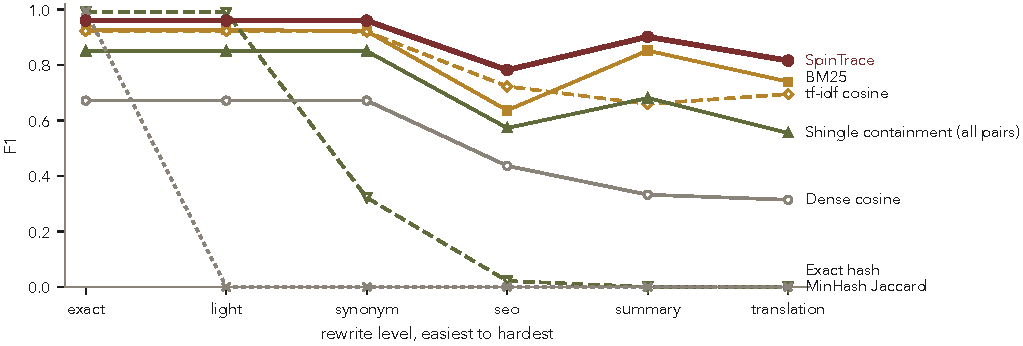
\includegraphics[width=0.98\textwidth]{figures/detection_f1_by_level.pdf}
  \caption{Detection F1 by rewrite intensity (test split). Shingle-based checks are near perfect while the words stay the same and collapse once they change.}
  \label{fig:f1}
\end{figure}

Table~\ref{tab:f1} and Figure~\ref{fig:f1} are the headline result. MinHash Jaccard goes from 0.990 on light edits to 0.322 on synonym spins and 0.021 on SEO rewrites; exact hash scores 0 after any edit. SpinTrace holds 0.960 through the synonym level and ends at 0.782 on SEO rewrites, 0.902 on summaries and 0.816 on round-trip translations, the best F1 at every level after light edits. On SEO rewrites its precision is 0.809 and its recall 0.756.

It loses at the easy end. Exact hash (0.995) and MinHash (0.992 and 0.990) beat its 0.960 on exact copies and light edits, and they cost almost nothing. SpinTrace's threshold is tuned for paraphrases, and the same-story negatives it still flags cost it precision (0.922) at every level. In a crawler the two should run together: the textbook check first, SpinTrace for what it lets through. BM25 comes within 0.05 on summaries (0.852), and full-document tf-idf flags slightly fewer facts-only articles (14.4\% against 15.6\%) while missing far more rewrites. On crawl hard negatives SpinTrace's false-positive rate is 0.007, while dense cosine flags half of them (0.502): to an embedding of the whole article, the same story looks like a copy.

\subsection{Ranking the original first}

SpinTrace ranks the true source first for 0.998 of test positives (MRR 0.998, Recall@20 1.000), and most baselines come close: full-document BM25 reaches 0.996, tf-idf cosine 0.993, shingle containment 0.987 and dense cosine 0.961. MinHash (0.526) and exact hash (0.239) only rank sources they can detect at all. Ranking the right source is easy for sparse methods on this corpus; the case for the rare-term query is in its cost.

\subsection{Index elimination and cost}

\begin{figure}[t]
  \begin{minipage}[t]{0.44\textwidth}
    \vspace{0pt}
    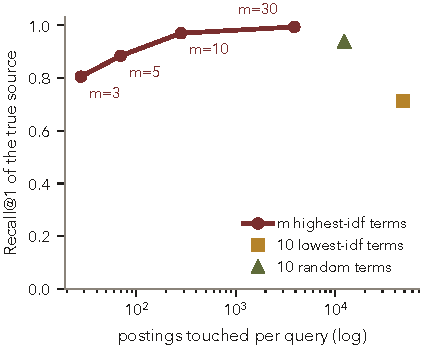
\includegraphics[width=\textwidth]{figures/index_elimination.pdf}
    \captionof{figure}{Recall@1 of the true source from the m highest-idf terms, against postings touched (test positives).}
    \label{fig:elim}
  \end{minipage}\hfill
  \begin{minipage}[t]{0.53\textwidth}
    \vspace{6pt}
    \small\setlength{\tabcolsep}{4pt}
    \captionof{table}{Cost per suspect, averaged over test items.}
    \label{tab:cost}
    \begin{tabularx}{\textwidth}{@{}lRRR@{}}
      \toprule
      \hrow \hd{Method} & \hd{ms} & \hdd{docs}{compared} & \hdd{postings}{touched} \\
      \midrule
      \ours SpinTrace & 23.2 & 20 & 8,293 \\
      Full-document query & -- & -- & 745,985 \\
      Shingle containment & 58.9 & 8,165 & -- \\
      tf-idf cosine & 12.0 & 8,165 & -- \\
      BM25 & 10.8 & 8,165 & -- \\
      Dense cosine & 1.4 & 8,165 & -- \\
      MinHash Jaccard & 0.1 & -- & -- \\
      Exact hash & 0.0 & -- & -- \\
      \bottomrule
    \end{tabularx}
  \end{minipage}
\end{figure}

Figure~\ref{fig:elim} varies the number m of rare terms in the query. Three terms find the source at rank 1 for 0.805 of positives while touching 28 postings; ten terms reach 0.970 with 282 postings; our setting of 30 reaches 0.994 with 3,891. Ten random terms reach 0.937 but touch 12,365 postings, and the ten most common terms reach only 0.713 with 48,375. The rarest terms are both the cheapest query and the most accurate one, which is the premise of Section~2 in one chart.

Table~\ref{tab:cost} gives cost per suspect. SpinTrace touches 8,293 postings, about 1\% of the 745,985 a full-document query touches, and only 20 documents reach the expensive comparison; all-pairs shingle containment compares every earlier document (8,165 on average) and takes 58.9\,ms. SpinTrace is not the fastest in wall-clock time, though: the baselines that compare precomputed vectors take 1.4 to 12.0\,ms against its 23.2\,ms.

\subsection{Originals and copies in search}

\begin{table}[t]
  \centering\small
  \caption{Search with and without g(d) (λ~=~0.1, tuned on dev). Synthetic: test queries from Wikinews titles, body-only relevance. Live: our 15 judged queries over the crawl, under each way of combining the two judges.}
  \label{tab:search}
  \begin{tabularx}{\textwidth}{@{}ll*{4}{R}@{}}
    \toprule
    \hrow \hd{Queries} & \hd{Setting} & \hd{P@10} & \hd{nDCG@10} & \hdd{original}{first} & \hdd{originals in}{relevant top 10} \\
    \midrule
    Synthetic & relevance only & 0.533 & 0.837 & 0.100 & 0.195 \\
    \ours & with g(d) & 0.524 & 0.886 & 0.526 & 0.203 \\
    \addlinespace[2pt]
    Live, either judge & relevance only & 0.933 & 0.973 & 0.867 & 0.927 \\
    \ours & with g(d) & 0.933 & 0.973 & 0.867 & 0.953 \\
    \addlinespace[2pt]
    Live, both judges & relevance only & 0.573 & 0.811 & 0.600 & 0.924 \\
    \ours & with g(d) & 0.560 & 0.803 & 0.600 & 0.963 \\
    \bottomrule
  \end{tabularx}
\end{table}

On synthetic queries, where we know which document is the original, g(d) puts the original first for 52.6\% of queries instead of 10\%, and nDCG@10 rises from 0.837 to 0.886; P@10 dips from 0.533 to 0.524 (Table~\ref{tab:search}). Our 15 judged live queries do not separate the rankings. When either judge's ``relevant'' counts, 93.5\% of judged results were relevant, so P@10 (0.933) and nDCG@10 (0.973) are identical with and without g(d), and the only change is the share of originals among the relevant top 10, from 0.927 to 0.953. When both judges must agree, nDCG@10 is slightly lower with g(d) (0.803 against 0.811).

\subsection{Human judgments of live flags}

Both of us labelled all 174 pairs that SpinTrace flagged in the live crawl. We judged blind: the judging page hides SpinTrace's score and verdict and the other judge's label. Live precision depends on how the two labels are combined: 0.845 if either judge says derived (our convention, and the lenient one), 0.437 if both must, and 0.738 on the 103 pairs we agreed on. We agreed on only 59\% of pairs (Cohen's kappa 0.123); Judge~1 called 103 derived and Judge~2 called 120. On search results agreement was 0.636 (kappa 0.161) over 154 judged results. Judge~1's not-derived pairs have much less exact overlap (median shingle containment 0.38, against 0.85 for derived pairs), which fits the sentence alignment matching independent coverage of one event.

\subsection{Documented farm pairs}

Two of four NewsGuard-documented pairs loaded from the Wayback Machine; for the other two the report does not name the originals. The New York Times original of a GlobalVillageSpace rewrite is retrieved first among 20,860 documents, verified at p~=~0.999 and traced. The Wired original of a TopGolf.kr page is also retrieved first but not verified (p~=~0.0): that page is AI title suggestions plus a reshaped deals list, and our verifier was trained on prose. Two pairs are anecdotes, not a measurement.

\subsection{Tracing translations}
\label{sec:xl}

A Hindi suspect has to be traced to its English source among all earlier English documents from other sites (about 8{,}800 on average, out of 20{,}900 in the English index); the source is among them unless the item is a source-absent negative. We report F1 for three derivative levels with the negatives pooled, and the false-positive rate (FPR) on three negative sets: an independent Hindi article on the same event, its 100-word version, and a derivative whose true source has been removed from the index. Thresholds are tuned on dev. Each baseline gets its best dev threshold: translate the suspect back to English with the LLM and run exact hash, MinHash, tf-idf, BM25 and the English SpinTrace on the result; multilingual dense cosine over every document; and retrieval from the suspect's Latin-script tokens alone, which shows whether the number, date and name bridge is needed.

\begin{table}[t]
  \centering\small
  \caption{Hindi to English, test split: F1 per derivative level and false-positive rate on three negative sets, with P@1 for the source. Back-translation baselines use English dev thresholds; rows with the threshold chosen on test and all confidence intervals are in \code{results/crosslingual\_detection.csv}.}
  \label{tab:xl}
  \footnotesize
  \setlength{\tabcolsep}{3pt}
  \begin{tabularx}{\textwidth}{@{}lRRRRRRR@{}}
  \toprule
  \hrow \hd{Method} & \hd{transl.} & \hd{SEO} & \hd{summary} & \hd{FPR same event} & \hd{FPR same event, 100 words} & \hd{FPR source absent} & \hd{P@1} \\
  \midrule
  \ours SpinTrace (anchors, no translation) & 0.860 & 0.852 & 0.818 & 0.100 & 0.220 & 0.000 & 0.993 \\
  Translate back, then SpinTrace & 0.906 & 0.771 & 0.753 & 0.060 & 0.120 & 0.000 & 0.993 \\
  Translate back, then tf-idf & 0.897 & 0.800 & 0.427 & 0.100 & 0.100 & 0.000 & 1.000 \\
  Translate back, then BM25 & 0.700 & 0.637 & 0.642 & 0.260 & 0.580 & 0.000 & 1.000 \\
  Translate back, then MinHash & 0.000 & 0.000 & 0.000 & 0.000 & 0.000 & 0.000 & 0.000 \\
  Translate back, then exact hash & 0.000 & 0.000 & 0.000 & 0.000 & 0.000 & 0.000 & 0.000 \\
  Multilingual dense cosine & 0.410 & 0.383 & 0.385 & 0.720 & 0.700 & 0.209 & 0.926 \\
  Latin-script tokens only & 0.327 & 0.381 & 0.163 & 0.820 & 0.720 & 0.290 & 0.480 \\
  \bottomrule
\end{tabularx}

\end{table}

SpinTrace on anchors reaches F1 \nXlTrans, \nXlSeo and \nXlSum on translations, SEO rewrites and summaries, and ranks the true source first for \nXlPone of all Hindi derivatives; the sets are small (\nXlTestN\ test originals per level), so the intervals in the CSV matter. Translating back and then running the English SpinTrace reaches \nBtSpinTrans, \nBtSpinSeo and \nBtSpinSum: a little lower, with overlapping intervals, so skipping the translation costs no accuracy on this set. Tf-idf and BM25 on the back-translation are weaker, most clearly on summaries (\nBtTfidfSum and \nBtBmSum), where a short brief shares less wording with its source after the round trip. Exact hash and MinHash score zero, as they must: a translation shares no shingles with its source. The embedding-only baselines are the weak ones: multilingual dense cosine reaches \nDenseTrans, \nDenseSeo and \nDenseSum and flags \nDenseFprSame of the same-event articles, and retrieval from Latin-script tokens alone reaches only \nLatinSum on summaries, so the bridge through numbers, dates and transliterated names does the work.

Where SpinTrace wins is cost, not accuracy, and the cost needs care. Retrieval takes about \nXlRetMs\,ms over about \nXlPostings\ postings with no LLM call and no embedding of the corpus. Verification then embeds the suspect's sentences and those of five candidates; with those embeddings cached a suspect costs \nXlMs\,ms in total, and with a cold cache about \nXlColdMs\,ms (measured separately on an idle machine; see \code{results/crosslingual\_cold\_cost.json}). Translating back costs about \nBtLlmSec\,s of LLM time per suspect before any detection, roughly \nSpeedup\ times more than our cold cost. Multilingual dense cosine is cheap per query (\nDenseMs\,ms) but needs every document embedded first, which took about fifteen minutes for the 20{,}860 English documents and grows with the corpus; the inverted index already exists.

\begin{table}[t]
  \centering\small
  \caption{Ablations for the Hindi path, test macro F1 over the three levels, each variant refit on dev. Full-system numbers differ from Table~\ref{tab:xl} because the ablation pools all levels.}
  \label{tab:xlabl}
  \footnotesize
  \begin{tabularx}{\textwidth}{@{}lRRRR@{}}
  \toprule
  \hrow \hd{Variant (refit on dev)} & \hd{macro F1} & \hd{P@1} & \hd{FPR same event} & \hd{postings touched} \\
  \midrule
  \ours Full system & 0.843 & 0.993 & 0.100 & 68483 \\
  No name anchors & 0.759 & 0.824 & 0.080 & 16849 \\
  No number anchors & 0.844 & 0.966 & 0.080 & 68411 \\
  No date anchors & 0.851 & 0.993 & 0.100 & 63177 \\
  Exact phonetic key only & 0.843 & 0.993 & 0.100 & 41698 \\
  Exact transliteration only (no fuzzy k-gram) & 0.791 & 0.865 & 0.060 & 17184 \\
  No source-language df check & 0.727 & 0.703 & 0.040 & 112852 \\
  30-day window instead of 7 & 0.855 & 0.993 & 0.040 & 68483 \\
  Dense retrieval, our verifier & 0.829 & 0.980 & 0.100 & -- \\
  No alignment signals & 0.408 & 0.966 & 0.960 & 68483 \\
  Anchor-overlap signals added & 0.751 & 0.993 & 0.120 & 68483 \\
  No retrieval score & 0.851 & 0.993 & 0.100 & 68483 \\
  \bottomrule
\end{tabularx}

\end{table}

Removing one thing at a time (Table~\ref{tab:xlabl}) shows which parts carry weight. Without the sentence-alignment signals macro F1 falls to \nAblNoAlign, so verification is essential and anchors alone cannot decide. Among the anchors, the source-language document-frequency check matters most (\nAblNoDf without it, against \nAblFull); it stops a name that is common in Hindi news but rare in our English crawl from acting as a strong anchor. Dropping name anchors costs more than dropping numbers (\nAblNoNames and \nAblNoNumbers), and exact transliteration without the fuzzy k-gram step gives \nAblTranslitExact. Dates change nothing at this scale (\nAblNoDates). Swapping our retrieval for dense retrieval with the same verifier gives \nAblDenseVerify, only a little behind, so on this corpus dense retrieval is nearly as good a candidate generator; what the index adds is that it needs no corpus-wide embedding and that every step can be read.

\paragraph{Length is not a shortcut}
\label{sec:length}
A hostile reading of Table~\ref{tab:xl} is that the negatives differ from the summaries in length rather than in derivation. We checked, and the worry is half right. Word count alone separates the Hindi summaries (median 117 to 120 words) from the same-event negatives (median 218 to 230 words) perfectly, with an AUC of 1.00 on both dev and test; translations (AUC 0.52) and SEO rewrites (0.76) are mostly not separable by length. So we generated a second same-event negative of about 100 words for every test original, and report the false-positive rate on both. SpinTrace flags \nXlFprShort of the short negatives against \nXlFprSame of the long ones: a small rise on 22 items with overlapping intervals. So the length gap did not decide the result, but the summary level is where it could have helped, and the zero on the long negatives should not be read as a guarantee. The short negatives are a test-only diagnostic: a threshold tuned on dev against the long negatives is exposed if it lets short ones through.

\paragraph{Other scripts: retrieval transfers, verification does not}
The same code, with the same dev thresholds and the multilingual sentence model, was tried on Tamil, Telugu and Bengali translations of 12 test originals each (Table~\ref{tab:xlother}). The generality check half failed, and the reason is informative. The anchors still retrieve the source: it is ranked first for \nTaPone, \nTePone and \nBnPone of the Tamil, Telugu and Bengali items, against \nDenseTaPone, \nDenseTePone and \nDenseBnPone for dense retrieval, which has no coverage of these scripts. Verification fails (F1 \nTaF, \nTeF and \nBnF), because the multilingual sentence model, to our knowledge, was not trained on these three languages, so sentence alignment carries no signal; we did not check the model card in this session. Where an embedding model does not cover a language, the index is the only part of the system that still works. These sets are tiny and are a negative generality result, not a benchmark.

\begin{table}[t]
  \centering\small
  \caption{Other scripts, test split, 12 originals per language. Retrieval from anchors transfers (first rows); the sentence-embedding verifier does not (last row). Intervals are in \code{results/crosslingual\_ranking.csv}.}
  \label{tab:xlother}
  \footnotesize
  \begin{tabularx}{\textwidth}{@{}lRRRR@{}}
  \toprule
  \hrow \hd{Measure} & \hd{Tamil} & \hd{Telugu} & \hd{Bengali} & \hd{Hindi, for comparison} \\
  \midrule
  \ours P@1, SpinTrace anchors & 0.417 & 0.667 & 0.917 & 1.000 \\
  P@1, multilingual dense & 0.083 & 0.083 & 0.083 & 0.980 \\
  P@1, Latin tokens only & 0.417 & 0.417 & 0.750 & 0.571 \\
  F1, SpinTrace verified as derived & 0.000 & 0.000 & 0.133 & 0.860 \\
  \bottomrule
\end{tabularx}

\end{table}

\paragraph{Live pages}
On the crawl itself we traced \nXlLiveSuspects\ Indian-language pages (\nXlLiveDeva\ in Devanagari) against English pages from the same days and earlier, and \nXlLiveFlagged\ were flagged, all Devanagari, a median \nXlLiveLag\ hours after the English page. Two of them are BBC Hindi articles traced to BBC News articles on another BBC domain, with the source credited: a bilingual outlet translating its own English reporting, which is the cross-language case in the wild. Others point to stories from the Times of India, The Independent and ThePrint, and one names the agency PTI; \nXlLiveCredit\ of the flagged pages credit their source. The flag rate is low for structural reasons: most Hindi stories have no English source in our crawl, outlets translating their own stories are filtered by the other-site rule, and same-event coverage is correctly rejected. A diagnostic that lets bilingual outlets match their own English pages (\nSameSiteSuspects\ pages of BBC and Hindustan Times in several scripts) flags \nSameSiteFlagged. Nobody has judged any of these, so we claim no live precision.

\subsection{Tracing mashups}
\label{sec:ms}

A mashup has to be traced to all of its sources. We score the predicted source set against the true one (precision, recall, F1 over sources and the share of mashups whose set is exactly right), on 759 rule-based splice mashups of two or three originals in known proportions and on the LLM mashups. Every method takes its best dev F1 among the thresholds that name a source for at most 10.6\% of the dev same-story articles and hard negatives, which is the false-source rate of the mid-term verifier as shipped, so no method buys recall by naming a source for everything. Baselines: the mid-term single-source pipeline; the same candidates above the threshold with no residual step (one-shot); MinHash LSH; and shingle containment against every earlier document, the strongest shingle method.

\begin{table}[t]
  \centering\small
  \caption{Mashups, test split: F1 of the predicted source set, by how the mashup was built. LLM mashups are those with both sources in the test split (a small set). Intervals are in \code{results/multisource\_detection.csv}.}
  \label{tab:ms}
  \footnotesize
  \setlength{\tabcolsep}{3pt}
  \begin{tabularx}{\textwidth}{@{}lRRRRRR@{}}
  \toprule
  \hrow \hd{Method} & \hd{all splices} & \hd{plain} & \hd{light edit} & \hd{synonyms} & \hd{SEO rewrite} & \hd{LLM mashups} \\
  \midrule
  \ours SpinTrace multi-source & 0.870 & 1.000 & 0.992 & 0.938 & 0.329 & 0.507 \\
  Shingle containment & 0.742 & 0.981 & 0.970 & 0.582 & 0.050 & 0.035 \\
  MinHash LSH & 0.188 & 0.384 & 0.292 & 0.008 & 0.000 & 0.000 \\
  Midterm single source & 0.117 & 0.209 & 0.182 & 0.057 & 0.000 & 0.000 \\
  One-shot multi & 0.117 & 0.209 & 0.182 & 0.057 & 0.000 & 0.000 \\
  \bottomrule
\end{tabularx}

\end{table}

% VERIFY direction of every comparison below against Tables tab:ms, tab:msrank, tab:msabl, tab:msctrl after the final run
SpinTrace recovers the source sets with F1 \nMsAll over all splices, against \nMsContAll for shingle containment and \nMsMidAll for the mid-term method, which cannot name more than one source and is capped well below that. On plain copy-and-paste splices shingle containment does about as well as we do (\nMsPlainCont against \nMsPlain) and is far cheaper; the gap opens when the blocks are reworded: \nMsSyn against \nMsSynCont for synonym-spun blocks and \nMsSeo against \nMsSeoCont for blocks taken from SEO rewrites. The one-shot baseline equals the mid-term one for a reason worth stating: a whole-document verifier passes a candidate only if it explains most of the suspect, and in a mashup of two or three sources at most one can, so one-shot almost never adds a second source. Recall of the second of two sources is \nMsSecondSpin for SpinTrace and \nMsSecondMid for the mid-term method, and of the third of three \nMsThirdSpin and \nMsThirdMid (Table~\ref{tab:msrank}). On the LLM mashups SpinTrace reaches F1 \nMsLlm against \nMsLlmCont for shingles; this set is small and its shares are unknown. Its precision there is \nMsLlmPrec\ but its recall only \nMsLlmRecall: under the false-source bar it names few of the sources, and those it names are right.

\begin{table}[t]
  \centering\small
  \caption{Share of true sources found, by the source's rank in the mashup (largest first), on test splices.}
  \label{tab:msrank}
  \footnotesize
  \setlength{\tabcolsep}{3pt}
  \begin{tabularx}{\textwidth}{@{}lRRRRR@{}}
  \toprule
  \hrow \hd{Method} & \hd{2 src: largest} & \hd{2 src: second} & \hd{3 src: largest} & \hd{3 src: second} & \hd{3 src: third} \\
  \midrule
  \ours SpinTrace multi-source & 0.875 & 0.812 & 0.742 & 0.721 & 0.705 \\
  Shingle containment & 0.729 & 0.630 & 0.653 & 0.484 & 0.458 \\
  MinHash LSH & 0.260 & 0.099 & 0.116 & 0.021 & 0.021 \\
  Midterm single source & 0.234 & 0.036 & 0.037 & 0.000 & 0.000 \\
  \bottomrule
\end{tabularx}

\end{table}

\begin{table}[t]
  \centering\small
  \caption{Mashup ablations, each variant retuned on dev under the same false-source bar; test numbers.}
  \label{tab:msabl}
  \footnotesize
  \setlength{\tabcolsep}{3pt}
  \begin{tabularx}{\textwidth}{@{}lRRRRR@{}}
  \toprule
  \hrow \hd{Variant (retuned on dev)} & \hd{F1 splices} & \hd{F1 SEO splices} & \hd{2nd of 2} & \hd{3rd of 3} & \hd{false source, same story} \\
  \midrule
  \ours Full (explain-away rounds) & 0.870 & 0.329 & 0.812 & 0.705 & 0.078 \\
  No residual query (one query) & 0.844 & 0.323 & 0.771 & 0.637 & 0.111 \\
  Residual without names, numbers, quotes & 0.867 & 0.304 & 0.807 & 0.700 & 0.078 \\
  Midterm whole-document verifier in the rounds & 0.118 & 0.000 & 0.036 & 0.000 & 0.111 \\
  \bottomrule
\end{tabularx}

\end{table}

The explain-away step is a smaller part of the result than we expected. Replacing the residual query with a single query for the whole suspect lowers splice F1 from \nMsAblFull\ to \nMsAblNoResid\ (Table~\ref{tab:msabl}): a single query already has the second source among its top five candidates for most two-source splices, so the residual query mainly helps the third source and lowers the false-source rate. What carries the result is the per-round verification criterion; putting the mid-term whole-document verifier inside the same rounds collapses F1. We state this because it would be easy to credit the rounds.

\begin{table}[t]
  \centering\small
  \caption{Controls: extra sources named for single-source rewrites (a correct answer is none), and sources named for same-story and hard-negative articles (a correct answer is none), on test.}
  \label{tab:msctrl}
  \footnotesize
  \setlength{\tabcolsep}{3pt}
  \begin{tabularx}{\textwidth}{@{}lRRRRRR@{}}
  \toprule
  \hrow \hd{Method} & \hd{extra: light} & \hd{extra: synonym} & \hd{extra: SEO} & \hd{extra: summary} & \hd{false: same story} & \hd{false: hard neg.} \\
  \midrule
  \ours SpinTrace multi-source & 0.000 & 0.000 & 0.000 & 0.000 & 0.078 & 0.033 \\
  Shingle containment & 0.000 & 0.000 & 0.000 & 0.000 & 0.178 & 0.000 \\
  MinHash LSH & 0.000 & 0.000 & 0.000 & 0.000 & 0.033 & 0.000 \\
  Midterm single source & 0.000 & 0.000 & 0.000 & 0.000 & 0.111 & 0.017 \\
  \bottomrule
\end{tabularx}

\end{table}

On the controls (Table~\ref{tab:msctrl}) SpinTrace never adds an extra source to a single-source rewrite, and names a false source for \nMsFalseSame\ of the same-story articles against \nMsFalseSameMid\ for the mid-term verifier as shipped. It loses on splices of LLM-paraphrased blocks, where its recall of single sources (64\% of SEO rewrites, 80\% of summaries) is below the mid-term verifier's, because the per-round criterion is stricter. It costs \nMsMs\,ms per suspect. On the crawl, 13 of 174 articles flagged by the single-source pipeline get two or more verified sources and none of 300 unflagged ones get any; in 6 of those 13 the two sources are one wire text printed by two outlets, which the output marks. These live results are unjudged.

\subsection{Mashups across languages: a prototype}
\label{sec:xlm}

The two new problems compose: a Hindi article stitched from two English originals. We tried the simplest thing that uses only parts we already have. The Hindi suspect is cut into blocks of \nXlmBlock\ sentences, about the size of the Hindi summaries the cross-language verifier was built for; each block is traced to an English source through the anchors; blocks that name the same source are merged, and a source's share is the fraction of sentences in its blocks. The explain-away rounds of Section~\ref{sec:ms} need a verifier fit on partial coverage of English sentences, which we have not built for Hindi. The block size and the probability threshold are tuned on dev under a 10\% false-source bar. The \nXlmN\ test items are Hindi splices of the translations and SEO rewrites of two originals from one split, so the sources and shares are exact.

\begin{table}[t]
  \centering\small
  \caption{Hindi splices, test split: source-set precision (P), recall (R) and F1 for all splices and by how the Hindi blocks were produced. Whole-text tracing can name at most one source.}
  \label{tab:xlm}
  \footnotesize
  \setlength{\tabcolsep}{2.5pt}
  \begin{tabularx}{\textwidth}{@{}lRRRRRRRRRR@{}}
  \toprule
  \hrow \hd{Method} & \hd{P} & \hd{R} & \hd{F1} & \hd{P transl.} & \hd{R transl.} & \hd{F1 transl.} & \hd{P SEO} & \hd{R SEO} & \hd{F1 SEO} & \hd{exact set} \\
  \midrule
  \ours Passage tracing (blocks, merged) & 1.000 & 0.620 & 0.765 & 1.000 & 0.754 & 0.860 & 1.000 & 0.500 & 0.667 & 0.387 \\
  Whole text, one source (dev threshold) & 1.000 & 0.275 & 0.431 & 1.000 & 0.396 & 0.567 & 1.000 & 0.167 & 0.286 & 0.000 \\
  Whole text, one source (shipped threshold) & 1.000 & 0.359 & 0.528 & 1.000 & 0.470 & 0.640 & 1.000 & 0.260 & 0.413 & 0.000 \\
  \bottomrule
\end{tabularx}

\end{table}

\begin{table}[t]
  \centering\small
  \caption{Controls for Hindi passage tracing, test split: extra sources named for single-source derivatives, the share of Hindi summaries whose source is found, and sources named for same-event articles of full and 100-word length (a correct answer is none).}
  \label{tab:xlmctl}
  \footnotesize
  \setlength{\tabcolsep}{3pt}
  \begin{tabularx}{\textwidth}{@{}lRRRRRR@{}}
  \toprule
  \hrow \hd{Method} & \hd{extra: transl.} & \hd{extra: SEO} & \hd{extra: summary} & \hd{summary found} & \hd{false: same event} & \hd{false: 100 words} \\
  \midrule
  \ours Passage tracing (blocks, merged) & 0.000 & 0.000 & 0.020 & 0.673 & 0.300 & 0.280 \\
  Whole text, one source (dev threshold) & 0.000 & 0.000 & 0.000 & 0.898 & 0.040 & 0.160 \\
  Whole text, one source (shipped threshold) & 0.000 & 0.000 & 0.000 & 0.918 & 0.100 & 0.240 \\
  \bottomrule
\end{tabularx}

\end{table}

% VERIFY the direction of each claim below against Tables tab:xlm and tab:xlmctl after the final run
Passage tracing recovers \nXlmRecall\ of the sources at precision \nXlmPrec\ (F1 \nXlmF), against \nXlmWholeRecall\ for tracing the whole text as one article (F1 \nXlmWholeF): a whole-text verifier does not pass an article that is only half copied, as in the English case. It is not a reliable detector, and the weaknesses come first. The exact source set is right for only \nXlmExact\ of the mashups. It names a false source for \nXlmFalseSame\ of the same-event articles, against \nXlmWholeFalseSame\ for the whole text; the dev rate was under the 10\% bar, so a threshold tuned at the edge of the bar did not carry over to test, on small sets. And it finds the source of fewer Hindi summaries (\nXlmSummaryFound against \nXlmWholeSummaryFound), because a three-sentence block of a summary carries too few anchors. We report it as a prototype showing that the two features compose, not as a result to build on; it costs about \nXlmMs\,ms per suspect.

\subsection{Format changes: a negative result}

We also tried the third kind of derivative the mid-term failed on, an article recast as a listicle or a question-and-answer page, where no sentences line up. We added order-free fact signals (idf-weighted overlap of names, numbers, dates and quotes, and fact-to-sentence coverage) and refit on dev. They did not help. The shipped verifier already handles rule-based listicles (F1 0.964) and Q\&As (0.943), because our reformattings keep whole sentences, and refitting with the fact signals lowers both to 0.931 and raises the false-positive rate on same-story articles from 0.156 to 0.300. The NewsGuard TopGolf.kr page, which motivated the experiment, is still retrieved first and still not verified by any variant. We report it as a negative result: a real format change by an LLM, with sentences rewritten, was not tested.


\subsection{Crawler correctness and politeness}

\begin{table}[t]
  \centering\small
  \caption{Crawl statistics from \code{crawl-report}. Every fetched URL is re-checked against the stored robots.txt.}
  \label{tab:crawl}
  \begin{tabularx}{\textwidth}{@{}Xr@{\hspace{2.2em}}Xr@{}}
    \toprule
    \hrow \hd{Measure} & \hd{Value} & \hd{Measure} & \hd{Value} \\
    \midrule
    Crawl time (hours), one process & 13.49 & Disallowed URLs fetched & 0 \\
    Page requests & 43,683 & Fetches audited against robots.txt & 43,674 \\
    robots.txt requests & 620 & URLs skipped by robots.txt & 512 \\
    Documents saved & 32,513 & Smallest gap to one host (s) & 0.29 \\
    Pages per minute & 54.0 & Requests under the 5\,s floor & 9 \\
    Hosts & 118 & Backoffs & 77 \\
    Median freshness (min, 968 articles) & 69.7 & Trap guards fired & 2,569 \\
    Exact / near duplicates & 792 / 1,099 & Duplicate rate & 0.0695 \\
    \bottomrule
  \end{tabularx}
\end{table}

Table~\ref{tab:crawl} summarises the crawl. No disallowed URL was fetched among 43,674 audited fetches, and 512 URLs were skipped because robots.txt disallowed them. The delay floor was not perfect: 9 requests came less than 5\,s after the previous one to the same host, the closest 0.29\,s apart. The last of them was at 23:45 on 6 October; the crawl report had exposed a race in the politeness check, which we fixed at 23:46.

\section{Limitations and next steps}
\label{sec:limits}

The boundary between ``same story'' and ``copied'' is where SpinTrace is weakest. Articles written from an original's facts and quotes alone are still flagged 15.6\% of the time, and recall on SEO rewrites is 0.76 at the dev-tuned threshold. The LLM rewrites closest to the ones NewsGuard tested are where SpinTrace misses most.

The live results say less about farms than we hoped. The crawl contained no actual farm sites; our seeds turned up aggregators and outlets that republish agency copy, and the live flags are mostly wire syndication (PTI, ANI, Reuters). When two outlets print the same agency story, SpinTrace credits whichever outlet we crawled first, because the agency itself is not crawled. Our only real farm cases are the two NewsGuard pairs.

Quote phrase matching, which we expected to be a key signal, turned out neutral. Retrieval with quote phrases finds the source first for 0.993 of positives against 0.994 without them, and removing quote overlap from the verifier leaves macro F1 at 0.896. Copies and independent coverage share quotes alike, since outlets quote the same speaker. The evidence is in names and numbers: removing their overlap drops macro F1 to 0.884 and raises the facts-only false-positive rate to 0.222. Our mined hard negatives share no text, so same-event pairs that share quotes are not yet tested.

Judge agreement was low (kappa 0.123 on live flags, 0.161 on search), so live precision is a range from 0.437 to 0.845, not a number. The synthetic test rewrites come from one 3B model; stronger models paraphrase more and would be harder. Publish dates are trusted, so a farm that backdates its pages escapes the earlier-only filter. Dropping the filter costs little in retrieval (Recall@1 0.989 against 0.993), but undated provenance mostly abstains on same-length rewrites and works mainly for summaries (Appendix, Table~\ref{tab:undated}). Scale is modest: one crawler process and 32.5k articles over 13.5 hours, of which the evaluation used about the first 16k.

\paragraph{Status of the mid-term roadmap} The mid-term report planned six items. English-to-Hindi derivatives are done and extended to three more scripts, and the harder evaluation is partly done: same-event negatives that share no quotes were already there, we added length-matched negatives and a second generator, but not rewrites from a stronger LLM or an external benchmark. Farm-aware crawling, agency-dateline recognition, learned signal weights from judged live pairs and adaptive recrawl scheduling were not attempted: we chose depth on two new detection problems over breadth. Multi-source mashups were not on the roadmap and were added.

\paragraph{Next steps} Stronger rewrite models and a real-translation benchmark; judged live pairs for both new features; a mashup path for Hindi suspects (a Hindi article stitched from two English originals, which would join the two new features); and a test at a scale where embedding every document is no longer affordable, which is where the anchor design should matter most.

\section{Work division and AI-use declaration}

\paragraph{Work division} Both of us wrote the plan, chose the track and the claim, and judged the live flags and search results independently. The commit history follows this split.

{\footnotesize
  \setlength{\tabcolsep}{0.9em}
  \begin{tabularx}{\textwidth}{@{}LL@{}}
    \toprule
    \hrow \hd{Nishita Kadali} & \hd{Pustak Pathak} \\
    \addlinespace[4pt]
    \textit{Crawler, IR core and detection signals} & \textit{Pipeline groundwork and evaluation} \\
    \midrule
    \begin{wdlist}
      \item Polite crawl loop, trap guards, frontier hardening
      \item Positional zoned index, tf-idf, BM25, MinHash, LSH
      \item Detection signals and the copy-graph scan
      \item Originality-aware search; inspect and trace commands
      \item Storage, export, re-crawl and run-all scripts; README
    \end{wdlist}
    &
    \begin{wdlist}
      \item URL normalisation, robots cache, frontier, extraction
      \item Candidate retrieval, verification and provenance stages
      \item Wikinews rewrites, hard negatives, NewsGuard pairs
      \item Baselines, ablations, scale run, charts, judge agreement
      \item Unit tests, critique notes, judging tool, demo web app
    \end{wdlist}
    \\
    \bottomrule
  \end{tabularx}
\par}

\paragraph{AI-use declaration}
\begin{itemize}[itemsep=0.25em]
  \item For the final we used Claude Code (Claude Opus 5.5 and Sonnet 5.5) again, and two helper agents in separate git worktrees: one wrote the cross-language path (\code{text\_indic.py}, \code{translit.py}, \code{kgram.py}, \code{detect/crosslingual.py}) and its evaluation, the other the multi-source path (\code{detect/multisource.py}) and its evaluation. We chose the problems, the claims and the experiments, reviewed the code, and ran a critique round whose notes are in \code{notes/}.
  \item Gemma 3 4B, run locally through Ollama, generated the Indian-language, back-translated and mashup test data; the pretrained multilingual MiniLM aligns sentences across languages.
  \item We used Claude Code (Anthropic, Claude Opus 5.5) as a coding agent throughout the build.
  \item From our plan and brief (\code{PLAN.md}, \code{CLAUDE.md}) it generated the package code under \code{spintrace/}, the tests, the command-line interface, the evaluation code and charts, the README, \code{PROGRESS.md} and the critique notes in \code{notes/}.
  \item We wrote the plan, the brief and the seed strategy, and reviewed the code and the results.
  \item Meta Llama 3.2 3B generated the mid-term's English SEO rewrites, summaries, round-trip translations and facts-only articles; all generated text is evaluation data only.
  \item The pretrained all-MiniLM-L6-v2 model serves verification and the dense baseline.
  \item No AI system labelled evaluation data: synthetic labels come from how the rewrites were built, hard negatives from a rule-based miner, and the mid-term's live labels from the two of us. The final's live results are unjudged.
\end{itemize}

\clearpage
\renewcommand{\refname}{References}
\begin{thebibliography}{9}
\small
\setlength{\itemsep}{0.2em}

\bibitem{ng2023} J.~Brewster, M.~Wang and C.~Palmer. Plagiarism-Bot? How low-quality websites are using AI to deceptively rewrite content from mainstream news outlets. \textit{NewsGuard Misinformation Monitor}, 24 August 2023. \url{https://www.newsguardtech.com/misinformation-monitor/august-2023}

\bibitem{ng2026} M.~Sadeghi et al. Tracking AI-enabled misinformation: AI content farm sites and top false claims generated by artificial intelligence tools. \textit{NewsGuard AI Tracking Center}, updated 23 June 2026, accessed 7 October 2026. \url{https://www.newsguardtech.com/special-reports/ai-tracking-center}

\bibitem{broder1997} A.~Z.~Broder. On the resemblance and containment of documents. In \textit{Proceedings of Compression and Complexity of Sequences (SEQUENCES '97)}, pages 21--29. IEEE, 1997.

\bibitem{manku2007} G.~S.~Manku, A.~Jain and A.~Das~Sarma. Detecting near-duplicates for web crawling. In \textit{Proceedings of the 16th International Conference on World Wide Web (WWW '07)}, pages 141--150. ACM, 2007.

\bibitem{heydon1999} A.~Heydon and M.~Najork. Mercator: A scalable, extensible web crawler. \textit{World Wide Web}, 2(4):219--229, 1999.

\bibitem{iir2008} C.~D.~Manning, P.~Raghavan and H.~Sch\"utze. \textit{Introduction to Information Retrieval}. Cambridge University Press, 2008.

\bibitem{robertson2009} S.~Robertson and H.~Zaragoza. The probabilistic relevance framework: BM25 and beyond. \textit{Foundations and Trends in Information Retrieval}, 3(4):333--389, 2009.

\bibitem{reimers2019} N.~Reimers and I.~Gurevych. Sentence-BERT: Sentence embeddings using Siamese BERT-networks. In \textit{Proceedings of EMNLP-IJCNLP 2019}, pages 3982--3992. ACL, 2019.

\bibitem{potthast2011} M.~Potthast, A.~Barr\'on-Cede\~no, B.~Stein and P.~Rosso. Cross-language plagiarism detection. \textit{Language Resources and Evaluation}, 45(1):45--62, 2011.

\bibitem{hagen2015} M.~Hagen, M.~Potthast and B.~Stein. Source retrieval for plagiarism detection from large web corpora: Recent approaches. In \textit{Working Notes of CLEF 2015}, 2015.

\bibitem{potthast2010} M.~Potthast, B.~Stein, A.~Barr\'on-Cede\~no and P.~Rosso. An evaluation framework for plagiarism detection. In \textit{Coling 2010: Posters}, pages 997--1005, 2010.

\end{thebibliography}

{\small
\textit{Data credits.} English Wikinews (CC BY 2.5, Wikinews contributors), read from the official Wikimedia dump; the live crawl from 36 seed outlets, of which only URLs and features are committed; NewsGuard-documented farm pages and their originals via the Internet Archive Wayback Machine; one Common Crawl CC-NEWS file (6 October 2026) for the scale experiment only; all-MiniLM-L6-v2 (Apache 2.0).\par}

\clearpage
\appendix
\renewcommand{\thetable}{A\arabic{table}}
\renewcommand{\thefigure}{A\arabic{figure}}
\setcounter{table}{0}
\setcounter{figure}{0}
\section*{Appendix}
\addcontentsline{toc}{section}{Appendix}

All numbers are on the test split, with anything tuned fit on dev.

\begin{table}[H]
  \centering\small
  \caption{SpinTrace precision, recall and share of positives traced to the correct source, per level.}
  \label{tab:pr}
  \begin{tabularx}{0.75\textwidth}{@{}l*{4}{R}@{}}
    \toprule
    \hrow \hd{Level} & \hd{Precision} & \hd{Recall} & \hd{F1} & \hd{Source correct} \\
    \midrule
    exact & 0.922 & 1.000 & 0.960 & 0.995 \\
    light & 0.922 & 1.000 & 0.960 & 0.995 \\
    synonym & 0.922 & 1.000 & 0.960 & 1.000 \\
    seo & 0.809 & 0.756 & 0.782 & 0.756 \\
    summary & 0.845 & 0.967 & 0.902 & 0.967 \\
    translation & 0.724 & 0.933 & 0.816 & 0.933 \\
    \bottomrule
  \end{tabularx}
\end{table}

\begin{table}[H]
  \centering\small
  \caption{Ablations: test macro F1 over the six levels, with the verifier refit on dev without the signal.}
  \label{tab:ablations}
  \begin{tabularx}{0.85\textwidth}{@{}l*{3}{R}@{}}
    \toprule
    \hrow \hd{Variant} & \hd{Macro F1} & \hd{FPR hard neg} & \hd{FPR facts-only} \\
    \midrule
    \ours Full & 0.896 & 0.007 & 0.156 \\
    minus rare-term cosine & 0.882 & 0.010 & 0.211 \\
    minus shingle containment & 0.892 & 0.007 & 0.167 \\
    minus alignment coverage & 0.884 & 0.007 & 0.211 \\
    minus alignment mean & 0.896 & 0.010 & 0.144 \\
    minus alignment order & 0.885 & 0.010 & 0.178 \\
    minus back coverage & 0.887 & 0.007 & 0.189 \\
    minus ordered coverage & 0.885 & 0.010 & 0.178 \\
    minus aligned word overlap & 0.900 & 0.007 & 0.144 \\
    minus quote overlap & 0.896 & 0.007 & 0.156 \\
    minus names and numbers overlap & 0.884 & 0.007 & 0.222 \\
    No embedding signals (IR signals only) & 0.802 & 0.007 & 0.444 \\
    Dense candidates instead of IR & 0.894 & 0.007 & 0.156 \\
    IR retrieval only, no verification & 0.595 & 0.242 & 0.767 \\
    \bottomrule
  \end{tabularx}
\end{table}

Removing aligned word overlap raises macro F1 slightly on test (0.900 against 0.896). It was added in our third critique round after cross-validation on dev only, and we kept it rather than tune on test.

\begin{table}[H]
  \centering\small
  \caption{Retrieval variants: share of test positives whose true source is ranked first and in the top 20.}
  \label{tab:variants}
  \begin{tabularx}{0.75\textwidth}{@{}l*{2}{R}@{}}
    \toprule
    \hrow \hd{Variant} & \hd{Recall@1} & \hd{Recall@20} \\
    \midrule
    \ours Rare terms + quote phrases & 0.993 & 1.000 \\
    Rare terms only (no quotes) & 0.994 & 1.000 \\
    No fact boost & 0.991 & 0.999 \\
    No date filter (dates untrusted) & 0.989 & 1.000 \\
    Rare terms, Porter stemming & 0.996 & 1.000 \\
    Dense retrieval & 0.961 & 1.000 \\
    Full-document tf-idf & 0.993 & 1.000 \\
    \bottomrule
  \end{tabularx}
\end{table}

With Porter stemming the rare-term query ranks the true source first for 0.996 of positives, against 0.993 for our unstemmed query with quote phrases, so stemming helps only at the margin.

\begin{table}[H]
  \centering\small
  \caption{Provenance without dates: coverage asymmetry on the known pair, margin 0.2.}
  \label{tab:undated}
  \begin{tabularx}{0.85\textwidth}{@{}l*{4}{R}@{}}
    \toprule
    \hrow \hd{Level} & \hd{n} & \hd{Suspect called derived} & \hd{Direction reversed} & \hd{Uncertain} \\
    \midrule
    exact & 190 & 0.000 & 0.000 & 1.000 \\
    light & 190 & 0.079 & 0.000 & 0.921 \\
    synonym & 190 & 0.000 & 0.000 & 1.000 \\
    seo & 90 & 0.167 & 0.033 & 0.800 \\
    summary & 90 & 0.956 & 0.000 & 0.044 \\
    translation & 45 & 0.178 & 0.022 & 0.800 \\
    hard negative & 301 & 0.053 & 0.030 & 0.917 \\
    facts-only & 90 & 0.267 & 0.000 & 0.733 \\
    \bottomrule
  \end{tabularx}
\end{table}

\begin{table}[H]
  \centering\small
  \caption{Scale: the same test items with the index grown to 24,501 documents by 3,637 CC-NEWS articles from the same days. Verifier and threshold not refit. False-positive rates at this size: originals 0.000, hard negatives 0.007, facts-only 0.156.}
  \label{tab:scale}
  \begin{tabularx}{\textwidth}{@{}l*{6}{R}@{}}
    \toprule
    \hrow \hd{Level} & \hd{Recall@1} & \hd{Recall@20} & \hd{Full-doc tf-idf Recall@1} & \hd{F1} & \hd{Postings touched} & \hd{Postings, full-doc query} \\
    \midrule
    exact & 1.000 & 1.000 & 1.000 & 0.960 & 9,698 & 811,153 \\
    light & 1.000 & 1.000 & 1.000 & 0.960 & 10,694 & 784,633 \\
    synonym & 1.000 & 1.000 & 1.000 & 0.960 & 6,747 & 817,589 \\
    seo & 0.989 & 1.000 & 0.978 & 0.789 & 9,948 & 747,305 \\
    summary & 0.956 & 1.000 & 0.978 & 0.902 & 21,650 & 399,229 \\
    translation & 0.956 & 1.000 & 0.956 & 0.816 & 12,022 & 683,412 \\
    \bottomrule
  \end{tabularx}
\end{table}

\begin{table}[H]
  \centering\small
  \caption{Per-domain integrity in the live crawl: share of a site's articles flagged as derived (top 10 sites).}
  \label{tab:domains}
  \begin{tabularx}{\textwidth}{@{}l*{3}{r}L@{}}
    \toprule
    \hrow \hd{Site} & \hd{Articles} & \hd{Flagged} & \hd{Share} & \hd{Main sources} \\
    \midrule
    devdiscourse.com & 692 & 20 & 0.029 & indiatimes.com (11); independent.co.uk (4); socialnews.xyz (2) \\
    theprint.in & 400 & 11 & 0.028 & indiatimes.com (4); hindustantimes.com (3); devdiscourse.com (1) \\
    independent.co.uk & 608 & 15 & 0.025 & abcnews.com (9); hindustantimes.com (2); france24.com (1) \\
    thehindu.com & 449 & 11 & 0.025 & socialnews.xyz (3); theprint.in (3); abcnews.com (2) \\
    indiatimes.com & 2,324 & 55 & 0.024 & devdiscourse.com (17); hindustantimes.com (13); indianexpress.com (10) \\
    latestly.com & 632 & 11 & 0.017 & dw.com (5); socialnews.xyz (3); abc.net.au (1) \\
    newsx.com & 316 & 5 & 0.016 & devdiscourse.com (4); theprint.in (1) \\
    scroll.in & 585 & 9 & 0.015 & theconversation.com (9) \\
    indianexpress.com & 548 & 8 & 0.015 & hindustantimes.com (2); indiatimes.com (2); devdiscourse.com (1) \\
    cbsnews.com & 339 & 4 & 0.012 & france24.com (3); abcnews.com (1) \\
    \bottomrule
  \end{tabularx}
\end{table}

These shares are flags, not judged derivatives; Section~5.5 gives the judged precision. Many of the source edges are outlets running the same agency story.

\begin{figure}[H]
  \centering
  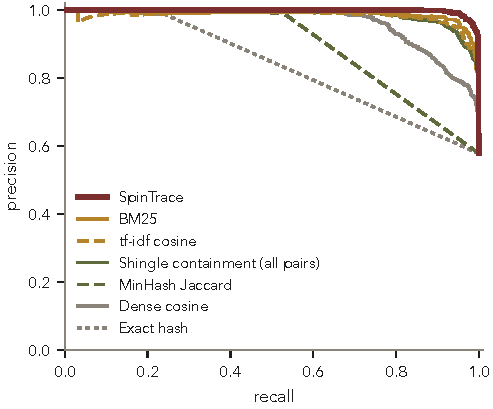
\includegraphics[width=0.55\textwidth]{figures/pr_curve.pdf}
  \caption{Precision and recall over all rewrite levels pooled (test), from each method's score.}
  \label{fig:pr}
\end{figure}

\end{document}
